\chapter{Background and Theory}
% This chapter should describe the theoretical background needed to understand
% and solve the problem. For instance, a description of the hardware platform
% or specific components involved in this assignment, definition of concepts
% that are important to understand the solution should be summarized here. Add
% citations to show sources whenever appropriate, LaTeX and bibliography
% managers make this easy.

% TODO: Write an introduction to ptxdist usage


\section{Operating Systems}
An operating system is a special piece of software that provides two important functions in a computer:
\begin{itemize}
  \item Managing the hardware resources.
  \item Providing a useful hardware abstraction layer for application programmers.
\end{itemize}
The core of the operating system is called the \emph{kernel} and runs in a privileged software mode that gives the kernel complete access to all hardware resources. The code running outside the kernel is often referred to as the \emph{user space} or the \emph{userland}, and has only restricted access to hardware. Because of this organization, all hardware-related activities necessary to run the operating system is performed by the kernel, and the user space programs only access hardware through \emph{system calls} in the kernel.\cite{modern-operating-systems}

\subsection{Device Drivers}
To more easily manage hardware devices with different characteristics, the kernel contains \emph{device drivers}. A device driver is a program that manages low-level hardware access to a particular device, providing a clean interface for the rest of the kernel programs.

\subsection{Kernel Modules}\label{sec:kernel-modules}
It is sometimes necessary to extend the functionality of the kernel, for instance if new hardware becomes available. While this could be achieved by modifying and rebuilding the kernel, a much more attractive alternative is to use \emph{kernel modules}, small programs that are loaded at runtime and extend the kernel with the needed functionality. Device drivers can be added as kernel modules.

\subsection{Related Terminology}
In addition to the concepts described above, several other terms are used in the context of operating systems:
\begin{itemize}
\item \textsl{Boot Loader:} The bootloader is a small program that runs before the operating system starts, and makes the necessary preparations to start the kernel.
\item \textsl{Linux Root Filesystem:} In Linux, the root filesystem is the filesystem available at the top-level directory. It is denoted with a forward slash, "/".
\end{itemize}
% TODO: Things to consider putting in here:
%   - Virtual address space (of a process)


\section{Linux}
TODO % TODO: Needs intro

\subsection{System calls}
TODO % TODO: Needs intro

\subsubsection{Reading and writing files}\label{sec:reading-and-writing-files}
Several system calls in Linux are related to file operations such as reading and writing. This section will introduce \texttt{open()}, \texttt{read()}, \texttt{write()}, \texttt{lseek()} and \texttt{close()}, available from the headers \texttt{fcntl.h} and \texttt{unistd.h}.

Before any file operations can be performed on a file, system resources needs to be allocated for the file, for instance with a call to \texttt{open()}:
\begin{verbatim}
  int open(const char *pathname, int flags);
\end{verbatim}
Here \texttt{pathname} is the absolute path to the file, and \texttt{flags} specify access modes such as read-only or read-write. On success, \texttt{open()} will return a file descriptor that is used as a handle when modifying the file with future system calls.

After opening a file with \texttt{open()}, the contents of the file can be read as individual bytes with \texttt{read()}:
\begin{verbatim}
  ssize_t read(int fd, void *buf, size_t count);
\end{verbatim}
Here \texttt{fd} is the file descriptor previously returned from \texttt{open()}, \texttt{buf} is a buffer where the file contents should be stored, and \texttt{count} is the number of bytes to read from the file. The returned value is the number of bytes that was read into \texttt{buf}. Note that \texttt{read()} gives no guarantee that the requested number of bytes has actually been read into \texttt{buf}. It is up to the application programmer to provide such guarantees by checking the return value.

In order to write write bytes to a file, it is possible to use the very similar function \texttt{write()}:
\begin{verbatim}
  ssize_t write(int fd, const void *buf, size_t count);
\end{verbatim}
Here the roles of the parameters are reversed: \texttt{buf} is a buffer containing the contents to write to the file, \texttt{count} specifies the number of bytes to write, and the value returned is the actual number of bytes written. As expected, \texttt{fd} is the file descriptor.

The functions \texttt{read()} and \texttt{write()} both perform their operations on the bytes located at a specific offset from the beginning of the file, called the \emph{file offset}. The file offset starts at the beginning of the file, and is incremented whenever a number of bytes is read or written by a file operation. To operate on bytes in a noncontiguous fashion, the offset needs to be changed with a call to \texttt{lseek()}:
\begin{verbatim}
  off_t lseek(int fd, off_t offset, int whence);
\end{verbatim}
Here the meaning of \texttt{offset} depends on the parameter \texttt{whence}. Three possible options are to specify the new offset directly, relative to the current offset, or relative to the end of the file.

After an application is done with a file, the resources associated with that file can be released by calling \texttt{close()}:
\begin{verbatim}
  int close(int fd);
\end{verbatim}
This will invalidate the file descriptor.\cite{linux-man-pages}


\subsubsection{Mapping files to memory}\label{mapping-files-to-memory}
Accessing a file in an arbitrary manner using the system calls described in \ref{sec:reading-and-writing-files} will involve many redundant calls to \texttt{lseek()}. A better alternative then is to map the file into the virtual address space of the process using \texttt{mmap()}, which will allow the file to be accessed with ordinary memory accesses:
\begin{verbatim}
  void *mmap(void *addr, size_t length, int prot, int flags,
                  int fd, off_t offset);
\end{verbatim}
This will map a number of \texttt{length} bytes from the file specified by the file descriptor \texttt{fd}, starting 
\texttt{offset} bytes from the beginning of the file. \texttt{addr} can be optionally used to give the kernel a hint as to where the mapping should be placed in virtual memory, or it can be \texttt{NULL}. \texttt{prot} is a bitfield specifying the memory protection of the mapping, and \texttt{flags} sets the visibility of updates to the mapping to other processes. An example of \texttt{mmap()} is shown in listing \ref{lst:mapping-file-to-memory}.
\lstset{style=lststyle-c}
\begin{lstlisting}[caption=Mapping the first 120 bytes of a file to memory,label=lst:mapping-file-to-memory]
void *map = mmap(NULL, 120, PROT_READ | PROT_WRITE, MAP_SHARED, fd, 0);
\end{lstlisting}

Updates to a memory mapped file might not become visible immediately. To synchronize a file with a memory map, the application should call \texttt{msync()}:
\begin{verbatim}
  int msync(void *addr, size_t length, int flags);
\end{verbatim}

After the application is done with the memory map, it may call \texttt{unmap()} to delete the mapping and release its associated resources: 
\begin{verbatim}
  int munmap(void *addr, size_t length);
\end{verbatim}
This will also cause the file to become synchronized with the memory map.



\section{Writing Device Drivers for Linux}
This section is a brief introduction to device driver development for the Linux kernel. It begins by explaining some practical details regarding driver development, then it highlights some important parts of the Linux kernel and common programming constructs, and finally it provides a brief outline on driver design. The main focus is on drivers implemented as kernel modules. For an explanation on the terminology used in this section, see section \ref{TODO}.
% TODO(optional): Update this introduction if necessary (e.g. if lots of new stuff was added)


\subsection{Programming in the Kernel}
Kernel modules are different from user space applications in several important ways, and there are some considerations to take into account when writing a module.

As a module is a part of the kernel, it runs in privileged mode with access to all hardware. A natural consequence of this is that bugs are much more serious. A module bug can easily crash the whole system, for instance by overwriting other parts of the kernel code in memory.
% TODO: Mention privileged mode in sec1

Again, because a module runs in privileged mode, it cannot be linked against any user space code. This includes the standard C library with all its nice functions such as \texttt{malloc()}, \texttt{strcmp()} and \texttt{printf()}. Instead, the module is linked against the kernel and has access to kernel routines.

Debugging is also different: the Linux kernel cannot be debugged with any user space debugger such as the GNU Debugger. Instead, the built-in kernel debugger must be used.

It is also worth mentioning that modules are linked against the kernel, meaning that the developer must have a kernel source tree available to build it against. The process of manually downloading, configuring and building a kernel source tree involves a fair amount of work, especially for a novice module programmer.


\subsection{Loading and Unloading Modules}
As explained in section \ref{sec:kernel-modules}, the kernel functionality can be extended by modules loaded at runtime. The following commands can be used to load and unload modules:
\begin{itemize}
  \item \texttt{insmod <module>} will load a module into memory and initialize it.
  \item \texttt{modprobe <module>} will load and initialize a module along with all its dependencies.
  \item \texttt{rmmod <module>} will perform cleanup and unload a module.
\end{itemize}
The modules are in control of their own initialization and cleanup processes. This is achieved by having each module define special initialization and exit functions that will be called whenever the module is loaded and unloaded respectively, as explained in the next section.


\subsection{A Simple Example}
The following example program illustrates the basic structure of driver module:
\lstset{style=lststyle-c}
\begin{lstlisting}
#include<linux/init.h>
#include<linux/module.h>

static int hello_init(void)
{
  printk(KERN_ALERT "Hello, world.\n");
}

static void hello_exit(void)
{
  printk(KERN_ALERT "Bye bye world, nice meeting you.\n");
}

module_init(hello_init);
module_exit(hello_exit);
\end{lstlisting}
This simple module uses the kernel function \texttt{printk()} to print messages when it is loaded and unloaded. Initialization and cleanup is done through the functions \texttt{hello\_init()} and \texttt{hello\_exit()} respectively. The important thing to note here is the functions \texttt{module\_init()} and \texttt{module\_exit()} at the last two lines: these are special macros that indicates to the kernel which functions to use for initialization and cleanup.

The included header files are included by almost all modules. Note that they are not system headers, but headers from the kernel source tree.


\subsection{Devices Files}
In Unix-like operating systems, user space applications access drivers through so-called \emph{device files} or \emph{special files}. These are similar to ordinary files in that they support many standard system calls for files, including the file operations described in section \ref{sec:reading-and-writing-files}. Notably, this is often true even for those drivers that do not provide access to storage devices at all. In any case, a driver provides its interface to the user space applications by implementing the needed system calls, and the implementation of those system calls constitutes a core part of the driver.

A device file contains information to identify the driver that owns it, namely a \emph{major} and a \emph{minor revision number}.

\textcolor{red}{(TODO: Write about how drivers registers device nodes in /dev)}


\subsection{Implementing Driver Operations}
We just explained that drivers are accessed through file operations that they define on a device file. This naturally begs the question of how those file operations are actually defined. In order to understand this, we need to look into how operations on files work in general for ordinary and special files alike.

The kernel uses the structure \texttt{struct file} from the kernel header \texttt{<linux/fs.h>} to manage open files. Some important fields of this structure are listed here:
\begin{description}
  \item[\texttt{mode\_t f\_mode;}] \hfill \\
    \texttt{f\_mode} is a bit field that stores the access mode of the file in the two bits \texttt{FMODE\_READ} and \texttt{FMODE\_WRITE}.
  \item[\texttt{loff\_t f\_pos;}] \hfill \\
    \texttt{f\_pos} is a 64-bit integer storing the current offset into the file.
  \item[\texttt{struct dentry *f\_dentry;}] \hfill \\
    \texttt{f\_dentry} points to a structure storing the directory entry of the file.   
  \item[\texttt{struct file\_operations *f\_op;}] \hfill \\
    \texttt{f\_op} points to a structure containing file operations to be used with the file.
\end{description}
The reader might be familiar with several of these file attributes. What is important, though, is the file operation structure associated with a file, \texttt{f\_op}. It is this structure that a driver uses to define the file operations of the device file. Below is a description of some fields in the structure \texttt{struct file\_operations}:
\begin{description}
  \item[\texttt{int (*open) (struct inode *, struct file *);}] \hfill \\
    Pointer to a function that is called whenever \texttt{open()} is called on the file.
  \item[\texttt{ssize\_t (*read) (struct file *, char \_\_user *, size\_t, loff\_t *);}] \hfill \\
    Pointer to a function that is called whenever \texttt{read()} is called on the file.
  \item[\texttt{ssize\_t (*write) (struct file *, const char \_\_user *, size\_t, loff\_t *);}] \hfill \\
    Pointer to a function that is called whenever \texttt{write()} is called on the file.
  \item[\texttt{loff\_t (*llseek) (struct file *, loff\_t, int);}] \hfill \\
    Pointer to a function that is called whenever \texttt{lseek()} is called on the file.
\end{description}
This structure reveals that drivers implement file operations on special files by providing a function pointer for each operation. These function pointers will likely point to internal driver functions.

\textcolor{red}{TODO: Write about how drivers register facilities and file operation structures}


\subsection{Handling Concurrency}
The driver is shared between the processes running on a system, and must correctly handle the scenario that two or more processes wants to use the driver at once. To share the driver between multiple processes, it might be necessary to manage resources on a per-process basis using data structures. In addition, the resources shared between the processes needs to be sufficiently protected with synchronization primitives to avoid race conditions.

As a driver registers its facilities, other parts of the kernel might try to use those facilities immediately. The driver needs to handle this case that some parts of the kernel try to use it before it is completely initialized.
% TODO: Expand this section when we have some experience about concurrency handling.


\subsection{Handling Errors}
When a driver registers a facility during initialization, there is no guarantee that the kernel is able grant the driver's request. The driver might still recover from such an event to provide either full or some partial service, but in the event that the driver is not able to continue, it should unregister all facilities previously registered successfully. This may require that the driver uses some sort of scheme to track which facilities was registered successfully and which failed. 
% TODO: Write about "facilities" somewhere.


\subsection{Mechanism versus Policy}
TODO % TODO: Write about "Mechanism vs Policy", as discussed by "Linux Device Driver" early in chapter 1.



\section{PTXdist}\label{sec:ptxdist}
PTXdist is a build system used to develop userland software for embedded platforms running Linux. It can control most parts of the build process:
\begin{itemize}
  \item Download package sources
  \item Extract package sources and apply patches
  \item Configure packages
  \item Build packages
  \item Create filesystem images
  \item Flash filesystem images to target
\end{itemize}
PTXdist builds the Linux kernel used along with the userland software.

\subsection{Project Setup}
Setting up a PXTdist project consists of the following steps:
\begin{itemize}
  \item Selecting a userland configuration.
  \item Selecting a hardware platform.
  \item Selecting a toolchain.
\end{itemize}
The userland configuration defines what user programs will be built for the target platform apart from the kernel, and the hardware platform defines the target platform of the build. The toolchain selected is the toolchain PTXdist should use when building. As PTXdist looks for toolchains in the /opt folder, selecting a toolchain is not always necessary.

\subsection{Building and Flashing}
After the project has been setup, the kernel and the user programs can be built with one simple command:
\lstset{style=lststyle-terminal}
\begin{lstlisting}
ptxdist go
\end{lstlisting}
This will build several filesystem images for the target platform containing the kernel and all userland programs specified by the userland configuration. PTXdist will automatically find out which packages needs to be built, and download them if necessary.

Finally, the images can then be flashed onto the target platform with the command:
\lstset{style=lststyle-terminal}
\begin{lstlisting}
ptxdist images
\end{lstlisting}
An illustration of how the PTXdist build process might be for a computer game is shown in figure \ref{fig:ptxdist-build-process}.

\begin{figure}[ht]\label{fig:ptxdist-build-process}
  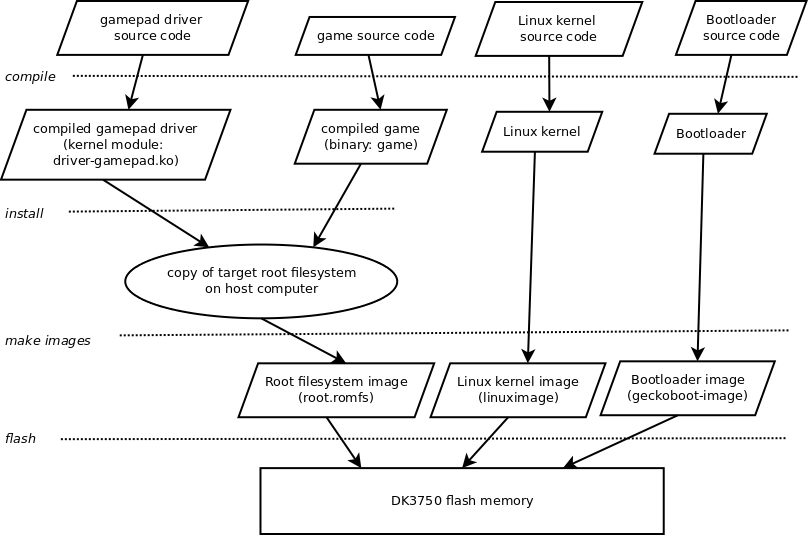
\includegraphics[width=\textwidth]{images/ptxdist_build_process.png}
  \caption{An example overview of a PTXdist build process for a computer game.}
\end{figure}

